% $Header: /project/cl/Root/CVS/talks/iowa08/talk.tex,v 1.3 2008/01/31 14:11:37 stump Exp $

\documentclass[11pt]{beamer}

\usepackage{tikz}
\usepackage{pgflibraryarrows}
\usepackage{pgflibraryshapes}
\usepackage{pgfbaseimage}
\usepackage{proof}
\usepackage{url}
\usepackage{code}

\newcommand{\Eq}[0]{\texttt{=}}
\newcommand{\Neq}[0]{\texttt{!=}}
\newcommand{\Qeq}[0]{\stackrel{?}{=}}
\newcommand{\bang}[0]{\texttt{!}}
\newcommand{\quant}[0]{\textit{Quant}}

\newcommand{\To}[0]{\Rightarrow}
\newcommand{\rn}[1]{\textsc{#1}}
\newcommand{\interp}[1]{[ \negthinspace [ #1 ] \negthinspace ]}

\newcommand{\seq}[3]{#1 \vdash #2 : #3}
%\newcommand{\aseq}[3]{ #2 : #3}
\newcommand{\aseq}[3]{ #1 \vdash #3}
%\newcommand{\aaseq}[3]{ #3}
\newcommand{\aaseq}[3]{ #1 \vdash #3}
\newcommand{\abseq}[3]{ #1 \vdash #3}


\mode<presentation>
{
  %\usetheme{Warsaw}
  % or ...

%\usetheme{IowaCity}
\usetheme{Edinburgh}
%\usetheme{Savannah}

%  \setbeamercovered{transparent}
  % or whatever (possibly just delete it)
}


\usepackage[english]{babel}
% or whatever

\usepackage[latin1]{inputenc}
% or whatever

\usepackage{times}
\usepackage[T1]{fontenc}
% Or whatever. Note that the encoding and the font should match. If T1
% does not look nice, try deleting the line with the fontenc.

\title[Verifying Imperative Abstractions]
{Verifying Imperative Abstractions with Dependent and Linear Types}

\author[Stump et al.]{Aaron Stump\inst{1} \and Evan Austin\inst{2}}

\institute[Computational Logic Center]
{
\inst{1}
  The University of Iowa
\and
\inst{2} The University of Kansas
\ \\
\ \\
Funding from NSF CAREER. 
}

% If you have a file called "university-logo-filename.xxx", where xxx
% is a graphic format that can be processed by latex or pdflatex,
% resp., then you can add a logo as follows:

% \pgfdeclareimage[height=0.5cm]{university-logo}{university-logo-filename}
% \logo{\pgfuseimage{university-logo}}



% Delete this, if you do not want the table of contents to pop up at
% the beginning of each subsection:
%\AtBeginSubsection[]
%{
%  \begin{frame}<beamer>
%    \frametitle{Outline}
%    \tableofcontents[currentsection,currentsubsection]
%  \end{frame}
%}


% If you wish to uncover everything in a step-wise fashion, uncomment
% the following command: 

%\beamerdefaultoverlayspecification{<+->}

\begin{document}

\date{\ }

\begin{frame}[plain]
  \titlepage
\end{frame}

\date{MVD '09}

\begin{frame}
  \frametitle{The \textsc{Guru} Approach}

\begin{center}
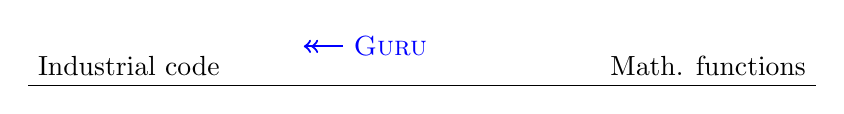
\begin{tikzpicture}
\draw (0,0) node[anchor=south west] {Industrial code} -- (10,0) node[anchor=south east] {Math. functions};
\draw[thick,->>,color=blue] (4,0.5) node[anchor=west,text=blue] {\textsc{Guru}} -- (3.5,0.5) ;
\end{tikzpicture}

\ 

\ \ \ \ \ \ \ \ \ \ \ \ \ \ \ \ \ \ \ 
\begin{tabular}{l}
\textcolor{blue}{General recursion} \\
\textcolor{blue}{Unaliased mutable state} \\
\textcolor{red}{Aliased mutable state [new!]} \\
No concurrency 
\end{tabular}

\end{center}

\end{frame}

\begin{frame}[containsverbatim]
  \frametitle{\textsc{Guru} at a High-Level}

\begin{itemize}

\item Pure functional language + logical theory.
\item Terms : Types.
\item Proofs : Formulas.
\item Declare types, write code:

{\footnotesize
\begin{verbatim}
(append [] l') = l'
(append x::l l') = x::(append l l')
\end{verbatim}
}

\item Prove theorems:
{
\footnotesize
\begin{verbatim}
Forall(A:type)(l l':<list A>). 
 {(length (append l l')) = (plus (length l) (length l'))}
\end{verbatim}
}
\item Define rich types:

\begin{itemize}
\item \texttt{<vec A N>} -- the type for vectors of \texttt{A}s of length \texttt{N}.
\item So \texttt{['a' 'b' 'c'] : <vec char 3>}.
\end{itemize}

\end{itemize}

\end{frame}

\begin{frame}
\frametitle{Functional Modeling for Imperative Abstractions}

\begin{itemize}
\item I/O, mutable arrays, cyclic structures, etc.
\item Do not fit well into pure FP.
\item Approach: functional modeling.
\begin{itemize}
\item Define a pure functional model (e.g., vectors for arrays).
\item Model is faithful, but slow.
\item Use during reasoning.
\item Replace with imperative code during compilation.
\item Use \emph{linear} (aka \emph{unique}) types to keep in synch.
\end{itemize}
\end{itemize}
\end{frame}

\begin{frame}
\frametitle{Example: Word-Indexed Mutable Arrays}

\begin{itemize}
\item Types: \texttt{<warray A N L>}.
\begin{itemize}
\item \texttt{A} is type of elements.
\item \texttt{N} is length of array.
\item \texttt{L} is list of initialized locations.
\end{itemize}

\item \texttt{(new\_array A N) : <warray A N []>}.

\item Writing to index \texttt{i}: 
\begin{itemize}
\item requires proof: \texttt{i < N}.
\item functional model: consume old array, produce updated one.
\item imperative implementation: just do the assignment.
\item array's type changes:  \texttt{<warray A N i::L>}.
\end{itemize}

\item Reading from index \texttt{i}:
\begin{itemize}
\item does not consume array.
\item requires proof: $\texttt{i}\in\texttt{L}$.
\end{itemize}
\end{itemize}
\end{frame}

\begin{frame}
\frametitle{Example: FIFO Queues}

\begin{itemize}
\item Mutable singly-linked list, with direct pointer to end.
\item \textbf{Aliasing!}
\item \textsc{Guru} approach: \emph{heaplets}.
\begin{itemize}
\item functionally model part of heap.
\item functional model: heaplet is list of aliased values.
\item implementation: no explicit heaplet.
\item functional model: aliases are indices into list.
\item implementation: aliases are reference-counted pointers.
\item caveat: not suitable for cyclic structures.
\end{itemize}
\end{itemize}
\end{frame}

\begin{frame}
\frametitle{Run-times}

\begin{itemize}
\item Linearity => memory deallocated explicitly.
\item Typing ensures memory safety.
\item \textsc{Guru}: no garbage collection!
\item Leads to good performance (cf. \textcolor{blue}{[Xian, Srisa-an, Jiang 08]}).
\end{itemize}

\begin{center}
Benchmark: push all words in ``War and Peace'' through 2 queues.

\ 

\begin{tabular}{|l|l|}
\hline
\textbf{Language} & \textbf{Wallclock time (s)} \\
\hline
\textsc{Haskell (Data.Queue)} & 29.8 \\
\textsc{Haskell (Data.Sequence)} & 5.6 \\
\textsc{OCaml} & 1.3 \\
\textsc{Guru} & 1.0 \\
\hline
\end{tabular}
\end{center}

\end{frame}


\begin{frame}
\frametitle{Conclusion}

\begin{itemize}
\item \textsc{Guru} combines FP, proofs, rich types.
\item Linear types + dependent types => verified imperative abstractions.
\item Mutable arrays, FIFO queues.
\item More examples to come.
\item Version 1.0 is close to release:

\ 

\begin{center}
\Large
\textcolor{blue}{\url{www.guru-lang.org}}
\end{center}

\end{itemize}

\end{frame}

\end{document}

